\documentclass[tikz,border=5pt]{standalone}

\usepackage{lmodern}
\usepackage{amsmath,amssymb}
\usepackage{xcolor}
\usepackage{tikz}
\usetikzlibrary{arrows.meta,calc,positioning}

% Colors
\definecolor{RedDeep}{RGB}{200,0,0}
\definecolor{BlueDeep}{RGB}{0,55,200}

% TikZ styles
\tikzset{
  >={Latex[length=2.6mm,width=2mm]},
  bell/.style={line width=0.9pt, draw=black},
  axisline/.style={line width=0.8pt, draw=black},
  eqsym/.style={font=\normalsize},
  smalllab/.style={font=\small},
  rednote/.style={RedDeep, font=\small},
  bluenote/.style={BlueDeep, font=\small},
}

% Reusable "bell with axis" pic
\tikzset{
  pics/bellaxis/.style args={#1}{
    code={
      % #1 = width of the bell (cm)
      \def\w{#1}%
      \def\h{1.1}%
      \def\axext{1.3}% axis extension to the right
      % bell curve
      \draw[bell]
        (-\w/2,0)
        .. controls (-0.25*\w,0) and (-0.18*\w,\h) ..
        (0,\h)
        .. controls (0.18*\w,\h) and (0.25*\w,0) ..
        (\w/2,0);
      % baseline + arrow
      \draw[axisline,-{Latex[length=2.2mm]}] (-\w/2,0) -- (\w/2+\axext,0);
    }
  },
  pics/bellaxis/.default=2.2
}

\begin{document}
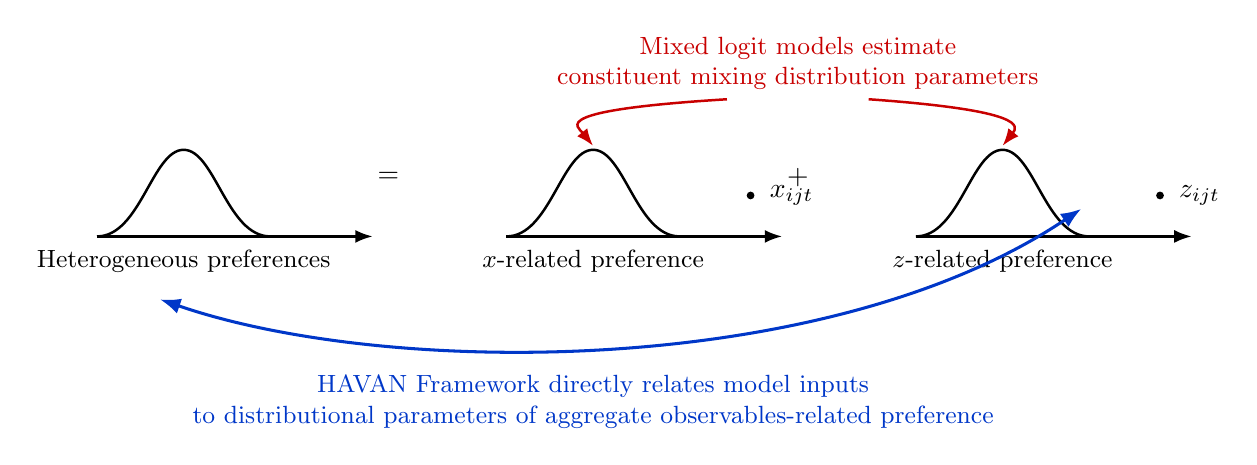
\begin{tikzpicture}[x=1cm,y=1cm]
  % Horizontal reference positions of the three groups
  \coordinate (L) at (0,0);
  \coordinate (M) at (5.2,0);
  \coordinate (R) at (10.4,0);

  % Bells
  \pic at (L) {bellaxis=2.2};
  \pic at (M) {bellaxis=2.2};
  \pic at (R) {bellaxis=2.2};

  % Captions under bells
  \node[smalllab, anchor=north] at ($(L)+(0,-0.05)$) {Heterogeneous preferences};
  \node[smalllab, anchor=north] at ($(M)+(0,-0.05)$) {$x$-related preference};
  \node[smalllab, anchor=north] at ($(R)+(0,-0.05)$) {$z$-related preference};

  % Equation symbols
  \node[eqsym] at ($(L)!0.5!(M)+(0,0.75)$) {$=$};
  \node[eqsym] at ($(M)!0.5!(R)+(0,0.75)$) {$+$};

  % Multiplying covariates (bullets with variables)
  \fill ($(M)+(2.0,0.52)$) circle (1.4pt);
  \node[anchor=west] at ($(M)+(2.12,0.52)$) {$x_{ijt}$};

  \fill ($(R)+(2.0,0.52)$) circle (1.4pt);
  \node[anchor=west] at ($(R)+(2.12,0.52)$) {$z_{ijt}$};

  % Top red annotation
  \node[rednote, align=center] (toptext) at ($(M)!0.5!(R)+(0,2.2)$)
    {Mixed logit models estimate \\ constituent mixing distribution parameters};

  % Red curved arrows from the text toward the two component bells
  \draw[RedDeep, line width=0.9pt, -{Latex[length=2.2mm]}]
    ($(toptext.south)+( -0.9,0.0)$) .. controls ($(M)+( -0.6,1.6)$) and ($(M)+( -0.2,1.4)$) ..
    ($(M)+( 0.0,1.15)$);
  \draw[RedDeep, line width=0.9pt, -{Latex[length=2.2mm]}]
    ($(toptext.south)+(  0.9,0.0)$) .. controls ($(R)+( 0.3,1.6)$) and ($(R)+( 0.2,1.4)$) ..
    ($(R)+( 0.0,1.15)$);

  % Bottom blue annotation (two lines)
  \node[bluenote, align=center] (bottomtext) at ($(M)!0.5!(R)+( -2.6,-2.1)$)
    {HAVAN Framework directly relates model inputs\\
     to distributional parameters of aggregate observables-related preference};

  % Long blue U-shaped double-headed arrow
  \draw[BlueDeep, line width=1.1pt, <->]
    ($(L)+(-0.3,-0.8)$)
    .. controls ($(L)+(2.6,-1.8)$) and ($(R)+(-2.2,-1.8)$) ..
    ($(R)+(1.0,0.35)$);

\end{tikzpicture}
\end{document}